\documentclass[sigconf]{acmart}

\title{Infinite Jest: An Elegant Hairball}
\author{
  K. Hunter Wapman
  \and
  Brian Lubars
  \and
  Carl Mueller
}
\date{\today}

%\documentclass[12pt]{article}
%\usepackage[margin=1in]{geometry}
\usepackage{amsmath}
\usepackage{enumitem}
\usepackage{graphicx}
\usepackage{listings}
% \usepackage{physics}
% \usepackage{subfig}
\usepackage{hyperref}
\usepackage{graphicx} % for pdf, bitmapped graphics files
\usepackage{caption}
\usepackage{subcaption}
\usepackage{wrapfig}
\usepackage[font={small}]{caption}
\usepackage{csquotes}
\usepackage{placeins}
\usepackage{xspace}

%\renewcommand\thesubsection{\alph{subsection}}

\newcommand{\infinitejest}{{\em Infinite Jest}\xspace}

%remove stupid copyright info
\settopmatter{printacmref=false}
\setcopyright{none}
\makeatletter
\def\@copyrightspace{\relax}
\makeatother

\captionsetup[subfigure]{aboveskip=2pt,belowskip=-1pt}
\captionsetup[table]{aboveskip=2pt,belowskip=-1pt}
\captionsetup[figure]{aboveskip=4pt,belowskip=0pt}
\setlength{\dbltextfloatsep}{8pt}
\setlength{\dblfloatsep}{8pt}
\setlength{\floatsep}{6pt}
\setlength{\textfloatsep}{8pt}

\begin{document}
\maketitle

\section{Introduction}

Storytelling has always been central to the human experience. Mediums for storytelling have evolved from an oral tradition to a range of genres with the written word and invention of the printing press. 
Novels of sufficient length may present complex social networks of character interactions, and thus provide opportunities to examine how literary social networks compare to ones we find in the real-world. 

Novels in particular also require the author to reveal the narrative world in pieces, leaving the reader to stitch together the complete picture and maintain an updated view as the story progresses. 
With this in mind, we may additionally examine the complex interplay between building the world and driving the plot forward. 
We may ask why author chose to structure the narrative a particular way. 
In \infinitejest, the story is split into sections which are ordered non-chronologically. 
The first few sections in the book are actually the last to occur chronologically!
Does this choice have a purpose reflected in the network structure which might make the book more or less comprehensible to the reader, or is it purely stylistic?

TODO: cite papers on narrative structures? 

In this work we seek to expand network analysis techniques for real-world social networks to examine artificial social networks in narratives.
Specifically, we extract and analyze a network of character interactions from \infinitejest, using character co-occurances to produce growing weighted undirected graph, with higher weights indicating more interactions.
We compare this narrative social network to properties exhibited by real-world networks, including a heavy-tailed degree distribution, the small-world property, inverse degree assortativity, and community structure. 
We confirm that centrality measures such as degree centrality and betweenness can recover the main characters, and comment on gender bias in the network.
Finally, we examine the narrative structure of \infinitejest by comparing the dynamics of the growing network in authored book-order versus chronological order.

\section{Background}

\subsection{Infinite Jest Book}

CHRONOLOGY

Sierpinski Gasket

“Certain kind of parallel lines are supposed to start converging in such a way that an "end" can be projected by the reader somewhere beyond the right frame. If no such convergence or projection occured to you, then the book's failed for you.” — DFW

Endnotes

\subsection{Why a Network?}

There are many possible definitions of an edge in a social network: dialogue, physical interactions, sentiment. 
We chose to present character co-mentions in the text as edges. 
This gives us the broadest view of a book as a network of character interactions, and additionally eases the burden of natural-language parsing because we can disregard all semantic information in the interactions.

\subsection{Questions..questions that need answering}

Would the book be more understandable if told in chronological order?

How is the narrative world structured? (static-network analysis)
Main characters: centrality measures
Small-world, community detection, assortativity


How does the structure evolve throughout the narrative? (dynamic analysis)
Chronological order vs. book order
Attachment: sparsification/densification?
Main character centralities over time


Why is the book structured this way?
Chronological vs. non-chronological
How does the structure impact the narrative?


\section{Related Work}

A quick search shows that we are not the first to mine networks from literary works and apply network analysis techniques.

In fact, there are a few interesting works which use data-driven analysis to evaluate hypotheses in literary analysis. 
Though it doesn't use networks, Reagan et al.'s uses NLP and sentiment analysis to confirm Kurt Vonnegut's rejected Master's thesus on emotional story arcs \cite{Reagan2016}. 
Analyzing 1,327 stories from Project Gutenberg, they find six core emotional trajectory arcs and compare modern popularity of stories for each arc evaluated by number of downloads.

Several social networks have been built from narratives. 
Alberich et al. (2002) build bipartite social network out of Marvel comic book character appearances in comic books, finding many similar characteristics to real-life scientific collaboration networks such as short distances and a power-law degree distribution tail with a cutoff \cite{2002marvel}. Notably, they find a lower clustering coefficient than expected in real networks.

Bonato et al. \cite{Bonato2016} compared networks for three books: {\em Twilight} by Stephanie Meyer, {\em The Stand} by Steven King, and J.K. Rowling's {\em Harry Potter and the Goblet of Fire}. 
They found the Chung-Lu model best fits the co-occurance networks.
Game of Thrones and Lord of the Rings have also been similarly analyzed \cite{GOT,ribeiro2016complex}.

%Meanwhile, Sack (1998) examines the emergence of global narrative structures from the local interactions of stable and unstable character triads, and discusses the implications as a generative mechanism for new story creation, particularly for dramas \cite{sack2013character}. Befriending and betrayal interactions between nodes represent an interesting potential dynamic for understanding narrative structure.

\infinitejest differs from the other narratives touched on in prior works because of its complexity, supposedly wide and in-depth wordview, and its unusual (non-chronological) structure. We therefore hope to find how this artificial social network compares to real social networks and to those previously analyzed. We suspect we may see statistics more similar to real-world social networks.

\section{Methods}

\subsection{Data Preprocessing}
\subsubsection{Data Source \& Preprocessing}
To generate analyzable text this project utilizes an existing `.mobi' file of \infinitejest. This file is put through a .mobi to HTML conversion to generate an HTML formatted file as well as a .mobi to raw text conversion. This enables the use of regular expressions to find and parse various text features automatically. Thus the HTML text is used to identify endnote locations such that simplified endnote tags can be inserted into the raw text file. Similarly, regular expressions are used to indentify where section breaks exist according to the section annotations given by the book Elegant Complexity \cite{carlisle_2007}. The raw text is split on these sections and saved into separate files. Likewise each endnote is saved into a separate file. In each of these files, we remove all inessential special characters (e.g. special quotes). As we employ the Python 3.7 standard, all text files are imported as unicode.

\subsubsection{Named Entitiy Recognition}

A major challenge with \infinitejest is the abundant use of pseudonyms and aliases of the 200+ characters in the novel. As our network uses characters as nodes, identifying named entities and their synonym coreference resolutions (not for pronouns) requires an extensive hand-engineered approach. We utilize the Named Entity Recognition (NER) parser of the Python library SpaCy \cite{spacy2} augmented with its own Matcher parser. By running the existing NER model on the text, we compare candidate entities generated from the NER parser with our own indetified character matches. Manually parsing over these results enables us to build an entity-synonym list that feeds into the Matcher in subsequent NER parses. This enables Spacy to indentify a large number of the pseudonyms and aliases and their locations within each section of the text.

CREATING GRAPHS examples

\subsubsection{Challenges and Considerations}
One major affront to the Matcher approach is the extensive use of pronoun coreferences. Similarly, the extensive use of dialog presents a challenge in identifying named entities since the the identification of the speaking character is often hidden. For example, in the following quote, two characters never explicitly mention each other but are refering to the same character, Bob.

Problems:
Point of View: who is “I”?
Reference vs Interaction
False positives
Disambiguation: Which John is John?
Pseudonyms
“Madame Psychosis” is a pseudonym of Joelle van Dyne
Hypergraph: “one of the Vaught sisters”

\begin{displayquote}
``\emph{\underline{I}} am really concerned about \emph{\underline{Bob}}"\\
``\emph{\underline{I}} am concerned about \emph{\underline{him}} too."\\
``What should \underline{\emph{we}} do about \underline{\emph{his}} problem?"
\end{displayquote}

This exchange would be overlooked by our approach. While there are some approaches for coreference resolution at this granularity, most are trained on models not well suited for the unstructured and informal style of David Foster Wallace's novel. As such, the use of named entities as nodes, and our methodology for identifying where they exist in text, enables the generation of a co-mention network. However, such a network may not perfectly capture true latent interaction structure of the book.

\subsection{Network Design}

\begin{figure*}[t]
    \centering
    \begin{subfigure}{0.4\textwidth}
        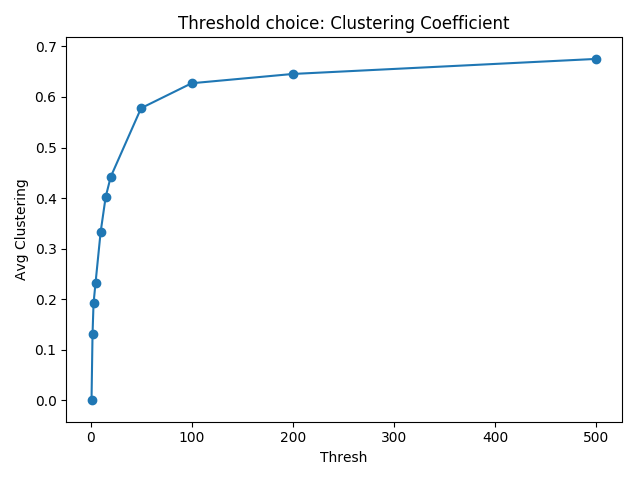
\includegraphics[width=1.\textwidth]{../data/plots/thresh_vs_avg_clustering.png}
        \caption{Clustering Coefficient vs. Threshold Size}
    \end{subfigure}
    ~
    \begin{subfigure}{0.4\textwidth}
        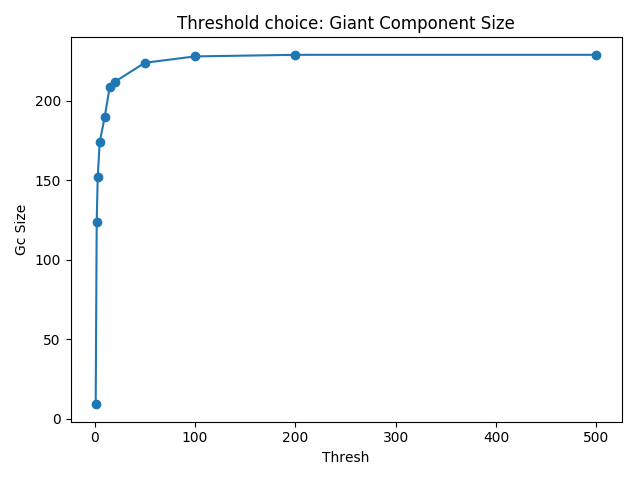
\includegraphics[width=1.\textwidth]{../data/plots/thresh_vs_gc_size.png}
        \caption{Giant Component Size vs. Threshold Size}
    \end{subfigure}
    \caption{Comparing threshold size effect on clustering coefficient and giant component size in order to determine the ideal threshold size.}
    \label{fig-threshold-size}
\end{figure*}

\subsubsection{Nodes and Edges}
Network nodes constitute each character identified in the set of found named entities. These were referenced against online resources to ensure proper coverage of the characters in the book. Edges in the book represent a co-mention between two entities in the text. A threshold number of tokens (words) under which the number of tokens between the mention of one entity and another determines if an edge is established. If the edge already exists, the weight is updated. The current entity $i$ is only matched with proceeding entities $j$ within this threshold. Once no match is found, the next available entity is checked for proceeding matches.

The threshold number of tokens is determined by a semi-objective measure of the effect of the threshold length on the average clustering coefficient and the giant component size (see Figure \ref{fig-threshold-size}). The intuition behind the use of these metrics is that we choose the minimum threhold length required to produce a large giant component and ample enough clustering best capturing the highly connected nature of characters in the novel. Our chosen threshold is 50 tokens.

\section{Static-Network Analysis}

\subsection{Statistics}

\subsubsection{Degree Distribution}
Average Degree

Power law? 
$$P(k) \sim k^{-\tau}$$
$$P(k) \sim k^{-\tau}10^{-k/c}$$

TODO: 'logarithmically bin data and perform a linear regression of Log(P(5)) on log(r) to get the power law fit

\subsubsection{Assortativity}

\subsubsection{Small World}
Comparison of diameter to real social networks?

\subsection{Modularity}

- talk about NMI
- talk about modularity

\subsubsection{Clustering}
 - compare against config model expectations?

 look at triangles, how many are closed/open, compare to expectations from a normal social network?

\subsection{Gender}

\section{Dynamic Analysis}

\subsection{Narrative}

\subsection{Sparsification vs Densification}

\section{Future Work}

Given more time and resources, there are several interesting questions to explore. We only ran our analysis with a single book, but it would be interesting to compare character interaction networks within and between different genres. For example, given a few dozen books, we could start to determine how \infinitejest's character network structure compare to other post-modern works, or how postmodern works differ from others like mysteries, historical fiction, fantasy, or short stories.

It would also be interesting to note if we can structurally identify common narrative techniques or plot devices -- for example, the climax, backstories, cliffhangers, plot twists, or stories-within-stories.

\section{Conclusion}

\bibliographystyle{ACM-Reference-Format}
\bibliography{references.bib}
\end{document}
